\documentclass[11pt]{elegantbook}
\definecolor{structurecolor}{RGB}{40,58,129}
\linespread{1.6}
\setlength{\footskip}{20pt}
\setlength{\parindent}{0pt}
\newcommand{\argmax}{\operatornamewithlimits{argmax}}
\newcommand{\argmin}{\operatornamewithlimits{argmin}}
\elegantnewtheorem{proof}{Proof}{}{Proof}
\elegantnewtheorem{claim}{Claim}{prostyle}{Claim}
\DeclareMathOperator{\col}{col}
\title{\textbf{Unsupervised Learning}}
\author{Wenxiao Yang}
\institute{Department of Mathematics, University of Illinois at Urbana-Champaign}
\date{}
\setcounter{tocdepth}{2}
\cover{cover.jpg}
\extrainfo{All models are wrong, but some are useful.}

% modify the color in the middle of titlepage
\definecolor{customcolor}{RGB}{32,178,170}
\colorlet{coverlinecolor}{customcolor}
\usepackage{cprotect}

\addbibresource[location=local]{reference.bib} % bib

\begin{document}

\maketitle
\frontmatter
\tableofcontents
\mainmatter

\chapter{Clustering}
General Goal of \textbf{Clustering Algorithm}:
\begin{enumerate}[$\circ$]
    \item the "similarity" of the objects in the same cluster is \underline{maximized} while
    \item the "similarity" of objects in different clusters is \underline{minimized}.
\end{enumerate}

\begin{definition}
    For a given set of objects $V = \{x_1, x_2, ... , x_m\}$, we call a \textbf{cluster $\mathbf{S_k}$} a subset of these objects, and we call a \textbf{clustering} the set of all $K$ clusters $\mathbf{\{S_1 ,S_2 , ... , S_k\}}$.
\end{definition}
\begin{example}
    Clustering of $\{x_1,x_2,x_3,x_4\}$: (1). $\{\{x_1,x_3\},\{x_2,x_4\}\}$; (2). $\{\{x_1,x_3\},\{x_1,x_2,x_4\}\}$; (3). $\{\{x_3\},\{x_2,x_4\}\}$.
\end{example}

\section{K-Means}
\subsection{Clustering Optimization Problem}
\begin{enumerate}
    \item \textbf{Input:}
    \subitem Desired number of clusters (ex: $K=3$)
    \subitem Dataset of $m$ objects $X=\{\vec{x}_1,\vec{x}_2,...,\vec{x}_m\}$, where each object $\vec{x}_i=(x_{i1},x_{i2},...\vec{x}_{in})$ has $n$ numerical attributes. (We can also think of $X$ as being an $m\times n$ matrix $X_{m\times n}$.)
    \item \textbf{Goal of k-Means:}
    \subitem Out of all possible clusterings of $\{S_1 ,S_2 , ... , S_K\}$ with $K$ clusters that can be made from the $m$ objects in $X$, find the optimal clustering $\{S_1^*,S_2^*,...,S_K^*\}$ that \underline{minimizes} the sum of the "distance" of each object and the centroid (the mean of the cluster that object is assigned to).
    \subitem Technically, we can write this as an optimization problem
    \begin{equation}
        \begin{aligned}
            \{S_1^*,S_2^*,...,S_K^*\}=\argmin_{S_1,S_2,...,S_K}\sum_{k=1}^K\sum_{x\in S_k}\|x-\mu_k\|^2\\
            \textnormal{Optimal Inertia}=\min_{S_1,S_2,...,S_K}\sum_{k=1}^K\sum_{x\in S_k}\|x-\mu_k\|^2\\
        \end{aligned}
        \nonumber
    \end{equation}
    Inertia measures how well a dataset was clustered by $K$-Means. It is calculated by measuring the distance between each data point and its centroid, squaring this distance, and summing these squares across one cluster. A good model is one with low inertia \underline{and} a low number of clusters ($K$).
\end{enumerate}
Find the clustering $\{S_1^*,S_2^*,...,S_K^*\}$ that provides a \underline{global minimum} is \textbf{NP-hard}.

We use a \underline{heuristic} algorithm to find a \underline{local minimum} is good enough.

\subsection{Lloyd's Algorithm}
\begin{enumerate}
    \item \textbf{Input:}
    \subitem Desired number of clusters (ex: $K=3$)
    \subitem Dataset of $m$ objects $X=\{\vec{x}_1,\vec{x}_2,...,\vec{x}_m\}$, where each object $\vec{x}_i=(x_{i1},x_{i2},...\vec{x}_{in})$ has $n$ numerical attributes. (We can also think of $X$ as being an $m\times n$ matrix $X_{m\times n}$.)
    \item \textbf{Algorithm:}
    \begin{enumerate}[$\bullet$]
        \item \textbf{\underline{Step 1:} Centroid Initialization Step}\\
        Randomly select $K$ centroids $\{\vec{\mu}_1,\vec{\mu}_2,...,\vec{\mu}_K\}$, where $\vec{\mu}_k=(\mu_{k1},\vec{\mu}_{k2},...,\vec{\mu}_{kn})$
        \item \textbf{\underline{Step 2:} Cluster Assignment Step}\\
        Assign each object $x_i$ in the dataset to it's \underline{closest} centroid (specifically the \textit{smallest squared euclidean distance})
        \item \textbf{\underline{Step 3:} Centroid Update Step}\\
        Find the \underline{mean} of each cluster created in step 2. These means are now the new \underline{centroids}.
        \item \textbf{\underline{Step 4:} Stopping Criterion}\\
        If the old centroids and the new centroids are the \underline{same}, stop the algorithm. Otherwise, go back to step 2.
    \end{enumerate}
    \item \textbf{Output:} Clustering with $K$ clusters $\{V_1,V_2,...,V_K\}$.
\end{enumerate}
Lloyd's algorithm is known as a \textbf{non-deterministic} algorithm because,
even with the same input, it can exhibit different behaviors on different runs.

\subsection{Benefits and Drawbacks}
\subsubsection*{Benefits}
\begin{enumerate}[$\bullet$]
    \item Fast algorithm.
    \item Computationally efficient.
    \item It scales well as the number of objects or attributes grows really large. (However, k-means is not great for "big data".)
    \item One of the easiest to understand.
\end{enumerate}
\subsubsection*{Drawbacks}
\begin{enumerate}[$\bullet$]
    \item Only works well with some types of data.\\
    The K-means algorithm works best for data when "the underlying clustering" of the data has the following properties:
    \begin{enumerate}[(1).]
        \item Each cluster has roughly the same number of objects;
        \item The clusters are spherical;
        \item The clusters have the same sparsity;
        \item There is good separation between the clusters;
        \item You know the right number of clusters to ask for;
        \item Attributes are numerical (non-categorical);
        \item Data does not have a lot of noise or outliers.
    \end{enumerate}
    (\textbf{Caveat:} Just because some of these assumptions are not met does not mean necessarily the algorithm will perform worse.)
    \item Need to know the "right" number of clusters to ask for in advance.
    (We use k-means elbow plot method)
    \item It is a non-deterministic algorithm.
\end{enumerate}

\subsection{Elbow Method}
\subsubsection*{Elbow Plot}
\begin{enumerate}
    \item For $k=1$ to $K$:
    \subitem[a] Cluster the data several times into $k$ clusters.
    \subitem[b] Calculate the average inertia of these resulting clusterings.
    \item Plot "k vs. average inertia".
\end{enumerate}
\begin{center}\begin{figure}[htbp]
    \centering
    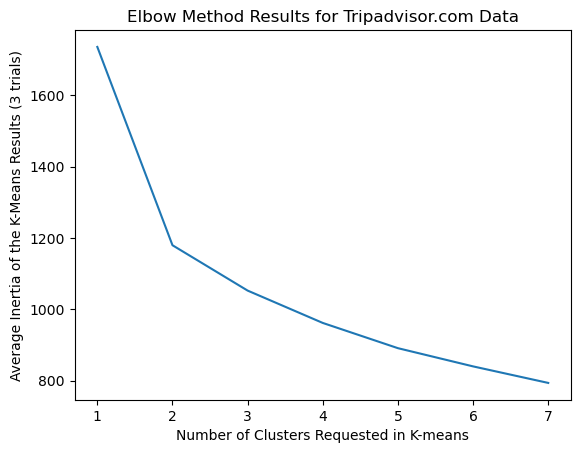
\includegraphics[scale=0.5]{elbow plot.png}
    \caption{Elbow Plot Example}
    \label{}
\end{figure}\end{center}
\subsubsection*{Interpretation of Elbow Plot}
\begin{enumerate}
    \item If there is not a dramatic elbow, then this suggests that either:
    \subitem 1. The dataset is \underline{not clusterable} or
    \subitem 2. K-means is not a suitable algorithm for detecting the underlying clusters.
    \item If there is a dramatic elbow, then this suggests that:
    \subitem 1. There is a clustering structure and
    \subitem 2. The k-means clustering algorithm is suggesting that there are about $K$ clusters where the plot levels off.
\end{enumerate}
In the example of the figure\\
1. We see a somewhat dramatic elbow in the plot. This suggests that there is some clustering structure in the dataset and that k-means is capable of identifying some clustering structure.

2. We see that that plot levels off dramatically at k=2 clusters. So this suggests that asking the k-means algorithm to return k=2 clusters will be the most insightful.

\section{Types of Clusters Definitions}
As we know the K-means algorithm can only work well with data that fulfills specific properties, we define some common \textbf{types of clusters} that could be considered in a numerical dataset to help introduce our new algorithms.

\begin{definition}[Well-Separated Cluster]
    A \textbf{well-separated cluster} defines a cluster only when the data contains natural clusters that are \underline{far apart from each other}. (This definition is vague in how far apart do clusters have to be.)
\end{definition}
Well-Separated Cluster can be non-spherical.
\begin{definition}[Density-Based Cluster]
    A \textbf{density-based cluster} defines a cluster as a \underline{dense} region of objects that is surrounded by a region of \underline{lower} density. (This definition is vague in how dense it needs to be considered a cluster.)
\end{definition}
Density-Based Cluster can have noise.

\begin{definition}[Graph-Based Cluster]
    \textbf{Graph-based cluster} is a group of objects that are \underline{connected} to one another, but have no \underline{connection} to objects outside the group. (This definition is vague in how do we decide objects are connected.)
\end{definition}
Graph-based cluster can be non-spherical and not well separated.

\begin{definition}[Contiguity-Based Cluster (a type of graph-based
    cluster definition)]
    In \textbf{contiguity-based cluster} (a type of graph-based
    cluster definition),  two objects are \underline{connected} only if they are within a \underline{specified distance} of one another.
\end{definition}
Contiguity-based clustering algorithms belong to spectral clustering.
\begin{center}\begin{figure}[htbp]
    \centering
    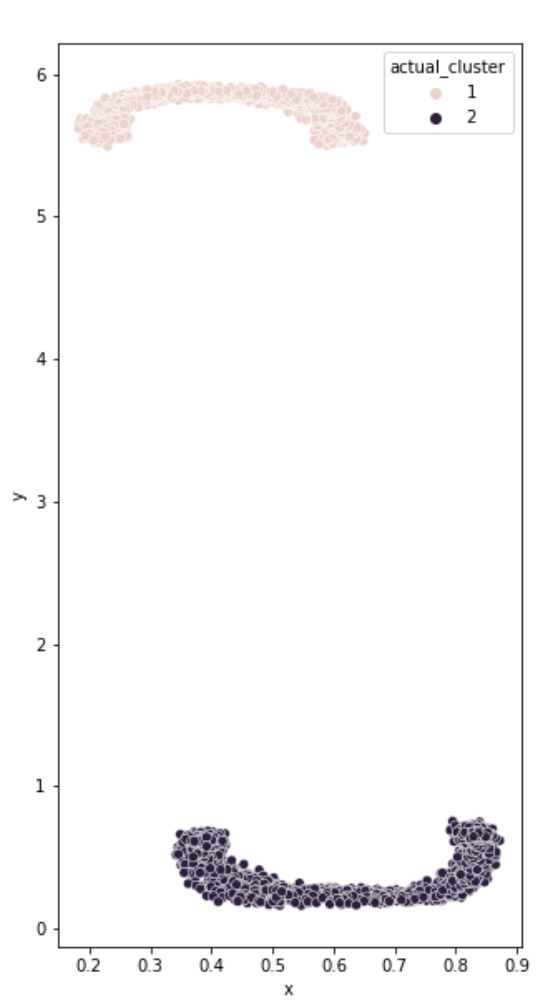
\includegraphics[scale=0.25]{well-separated.png}
    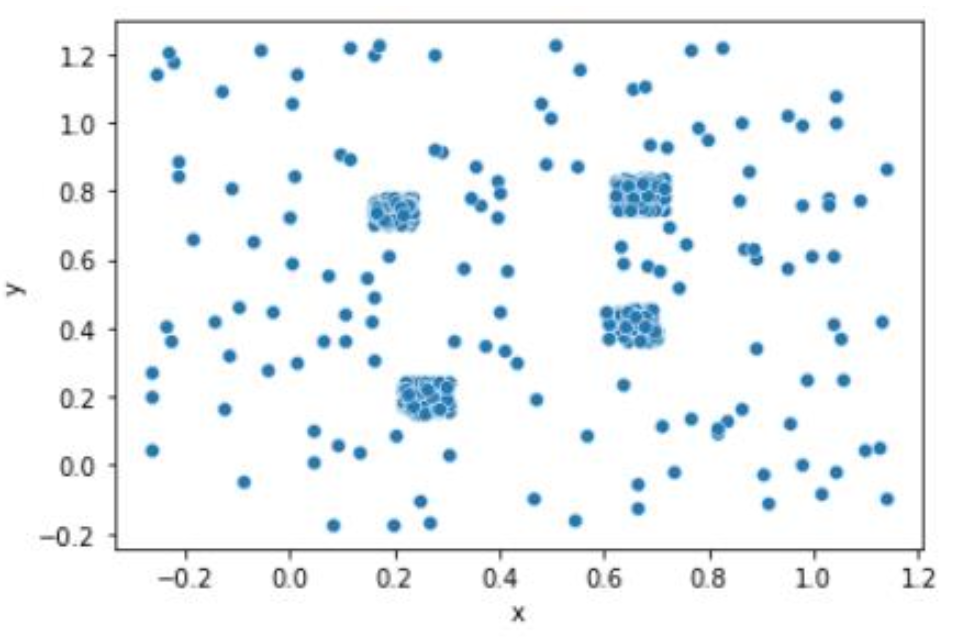
\includegraphics[scale=0.25]{density-based.png}
    \caption{(1). Well-Separated Cluster; (2). Density-Based Cluster}
    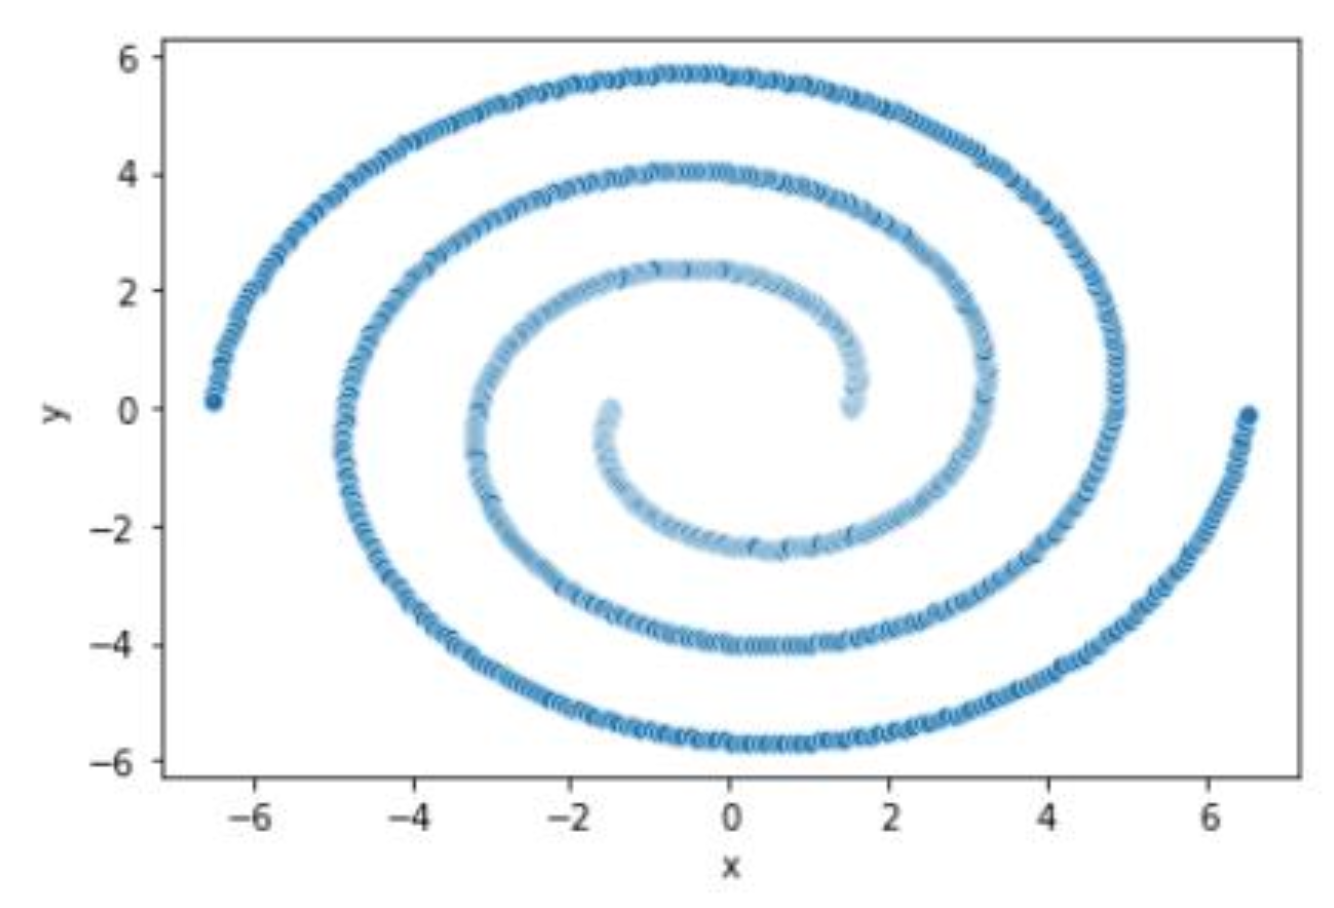
\includegraphics[scale=0.2]{Contiguity-based.png}
    \caption{Contiguity-Based Cluster}
\end{figure}\end{center}

\begin{definition}[Prototype-Based Cluster]
    A \textbf{prototype-based cluster} defines a cluster as a set of objects in which each object is closer (or more similar) to the \underline{prototype} that defines the cluster than to the \underline{prototype} of any other cluster.
\end{definition}



















\end{document}